\chapter{Tesztelési eredmények}

\thispagestyle{fancy}
\pagestyle{fancy}

Szabó Patrícia témavezetőmnek köszönhetően az kész projektemet sikerült az egyetem hallgatóival leteszteltetni.
A teszt eredményeit a User Experience Questionnaire, röviden UEQ adat elemző eszközzel, valamint a System Usability Scale azaz SUS-al lett kiértékelve. 
 
\section{Demográfiai adatok}
A demográfiai adatok a \ref{tab:demografia} táblázatban láthatók. A hallgatók kiválasztásánál különös figyelmet fordítottunk arra, hogy a lehető legszélesebb körből válogassunk, biztosítva ezzel a minta reprezentativitását. A sokszínű csoport segít abban, hogy mérésünk eredményei minél pontosabbak és általánosíthatóbbak legyenek. Célunk volt, hogy különböző korcsoportokból, különböző iskolai végzettséggel rendelkező egyéneket, valamint különböző technológiai jártasságú résztvevőket vonjunk be, ezáltal csökkentve az esetleges torzítások hatását. Ennek eredményeként úgy véljük, hogy a gyűjtött adatok megbízhatóan tükrözik a valóságot, és hasznos következtetéseket vonhatunk le belőlük.

\begin{table}[!h]
    \caption{Demográfiai adatok}
    \label{tab:demografia}
    \resizebox{\linewidth}{!}{%
    \begin{tabular}{ccccccc} % specify the number of columns
    \hline
    \multicolumn{1}{c}{\textbf{ID}} & 
    \multicolumn{1}{c}{\textbf{Korcsoport}} & 
    \multicolumn{1}{c}{\textbf{Nem}} & 
    \multicolumn{1}{c}{\textbf{Legmagasabb iskola}} & 
    \multicolumn{1}{c}{\textbf{Techn. Járt.}} & 
    \multicolumn{1}{c}{\textbf{Elsődleges játékhoz}} & 
    \multicolumn{1}{c}{\textbf{Oktatásban töltött évek száma}} \\ \hline
    
    1 & 18-24 & Férfi & Középiskola & Haladó & Asztali számítógép & 13 \\
    2 & 25-34 & Férfi & Középiskola & Középhaladó & Laptop & 18 \\
    3 & 18-24 & Férfi & Technikus & Kezdő & Laptop & 14 \\
    4 & 18-24 & Férfi & Technikus & Haladó & Asztali számítógép & 13 \\
    5 & 18-24 & Férfi & Középiskola & Középhaladó & Asztali számítógép & 16 \\
    6 & 18-24 & Férfi & Középiskola & Kezdő & Asztali számítógép & 14 \\
    7 & 18-24 & Férfi & Középiskola & Középhaladó & Asztali számítógép & 15 \\
    8 & 18-24 & Férfi & Középiskola & Haladó & Asztali számítógép & 16 \\
    9 & 18-24 & Férfi & Középiskola & Haladó & Asztali számítógép & 13 \\
    10 & 25-34 & Férfi & Mesterfokozat & Szakértő & Okostelefon & 20 \\
    11 & 25-34 & Férfi & Főiskolai diploma & Szakértő & Asztali számítógép & 17 \\
    
    \hline
    \end{tabular}%
    }
    \end{table}

\section{UEQ - User Experience Questionnaire}


Az \textit{User Experience Questionnaire} (UEQ) egy gyakran használt eszköz, amely lehetővé teszi a termékek és szolgáltatások használói élményének mérését. Az UEQ kifejezetten úgy lett kialakítva, hogy gyorsan és hatékonyan nyújtson visszajelzést a felhasználói élmény különböző aspektusairól, mint például a használhatóság, az esztétika és az érzelmi hatások.

\subsection{Kérdőív felépítése és dimenziói}

Az UEQ kérdőív 26 tételből áll, amelyeket hat különböző dimenzióra osztanak:

\begin{itemize}
    \item \textbf{Vonzalom (Attractiveness)}: Az általános benyomás és az érzelmi reakció a termékre vagy szolgáltatásra.
    \item \textbf{Megértés (Perspicuity)}: A termék vagy szolgáltatás használatának egyszerűsége és könnyű megértése.
    \item \textbf{Hatékonyság (Efficiency)}: A feladatok gyors és hatékony végrehajtásának képessége.
    \item \textbf{Szervezettség (Dependability)}: Az irányítás érzete és a rendszer kiszámíthatósága.
    \item \textbf{Stimuláció (Stimulation)}: A termék vagy szolgáltatás által nyújtott inspiráció és motiváció.
    \item \textbf{Újdonság (Novelty)}: Az innováció érzete és a termék vagy szolgáltatás újszerűsége.
\end{itemize}

A következő megállapításokat tehetjük a különböző értékelésekről és azok szerepéről a mi esetünkben:

\begin{itemize}
    \item \textbf{Semleges értékelés (-0,8 és 0,8 között):} Ez a tartomány a skála viszonylag semleges megítélését jelzi. Ilyen értékek esetén az eredmények nem mutatnak kiemelkedő pozitív vagy negatív irányt.
    
    \item \textbf{Pozitív értékelés (> 0,8):} Ezek az értékek pozitív megítélést jelentenek. A mi esetünkben, ha a skálán +0,8 feletti értékek szerepelnek, az azt jelzi, hogy a vizsgált jellemzők kedvezőek és pozitív benyomást keltenek.
    
    \item \textbf{Negatív értékelés (< -0,8):} Ezek az értékek negatív értékelést tükröznek. Ha a skála -0,8 alatti értékeket mutat, az a vizsgált jellemzők kedvezőtlen megítélésére utal.
    
    \item \textbf{Skálatartomány:} A skála értékeinek teljes tartománya -3 (nagyon rossz) és +3 (nagyon jó) között mozog. A valós alkalmazásokban a legtöbb esetben a -2 és +2 közötti értékekkel találkozunk, mivel az extrém válaszok ritkán fordulnak elő.
\end{itemize}

\subsection{Kiértékelés}
\begin{table}[h]
    \centering
    \caption{UEQ skála, Átlag és változat}
    \begin{tabular}{|l|c|c|}
        \hline
        \textbf{Skála} & \textbf{Átlag} & \textbf{Változat} \\ \hline
        Kellem & 1.167 & 0.53 \\ \hline
        Áttekinthetőség & 2.364 & 0.74 \\ \hline
        Hatékonyság & 0.750 & 0.59 \\ \hline
        Megbízhatóság & 1.136 & 1.08 \\ \hline
        Ösztönzés & 1.159 & 0.63 \\ \hline
        Újszerűség & 0.500 & 0.78 \\ \hline
    \end{tabular}
    \label{tab:ueq_scales}
\end{table}

\begin{figure}[h]
    \center
    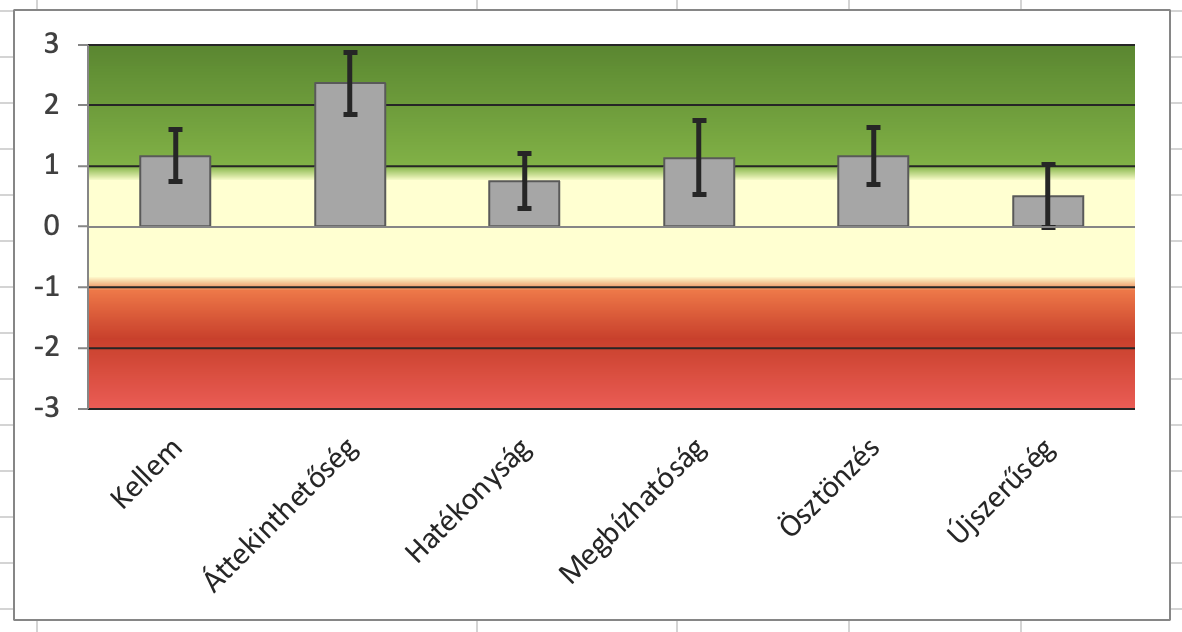
\includegraphics[width=0.75\textwidth]{img/UEQ_diagram.png}
    \caption{UEQ diagram eredmények}
    \label{diag:ueq}
\end{figure}

A \ref{tab:ueq_scales} táblázat adatai alapján, a hatból 4 dimenzióban jól teljesített  programom, Áttekinthetősségben kiemelkedően, és csak a Hatékonyság és az Újszerűség az, ahol neutrálisak az értékek. A \ref{diag:ueq}. ábra jól szemlélteti ezt. 


A UEQ skáláit a következő két fő kategóriába sorolhatjuk: pragmatikus minőség (amely magában foglalja az Áttekinthetőséget, Hatékonyságot és Megbízhatóságot) és hedonikus minőség (Ösztönzés és Újszerűség). Míg a pragmatikus minőség a feladatokhoz kapcsolódó minőségi szempontokat értékeli, addig a hedonikus minőség a nem feladatorientált minőségi tényezőkre fókuszál.

A \ref{tab:pragmatic_hedonic_quality}. táblázatban a \textit{kellemes} a három \textit{pragmatikus} és a két \textit{hedonikus} minőség szempont átlagértéke kerül kiszámításra. 

\begin{table}[h]
    \centering
    \caption{Pragmatikus és hedonikus minőségek}
    \begin{tabular}{|l|c|}
        \hline
        \textbf{Kategória} & \textbf{Érték} \\ \hline
        Kellem & 1.17 \\ \hline
        Pragmatikus minőség & 1.42 \\ \hline
        Hedonikus minőség & 0.83 \\ \hline
    \end{tabular}
    \label{tab:pragmatic_hedonic_quality}
\end{table}

Megvizsgálva az értékeket, boldogan tapasztaltam, hogy mind a három csoportban pozitív eredményt érhettem el, noha a Hedonikus értékekben épp csak megütöttem a 0.83-al. Ezt a \ref{diag:pragmatic_hedonic}. ábra is tökéletesen szemlélteti. 

Kimagaslóan jó eredményem lett a pragmatikus minőségekből, amiből én arra következtetek, hogy a programom a feladatát megfelelően végzi el. 

Amin a jövőben javíti kell a memória játékon, az az újszerűség, mely a hedonikus minőségen is javítani tud. Ezt valamilyen innovatív megoldással tudnám a legkönnyebben elérni. 

\begin{figure}[h]
    \center
    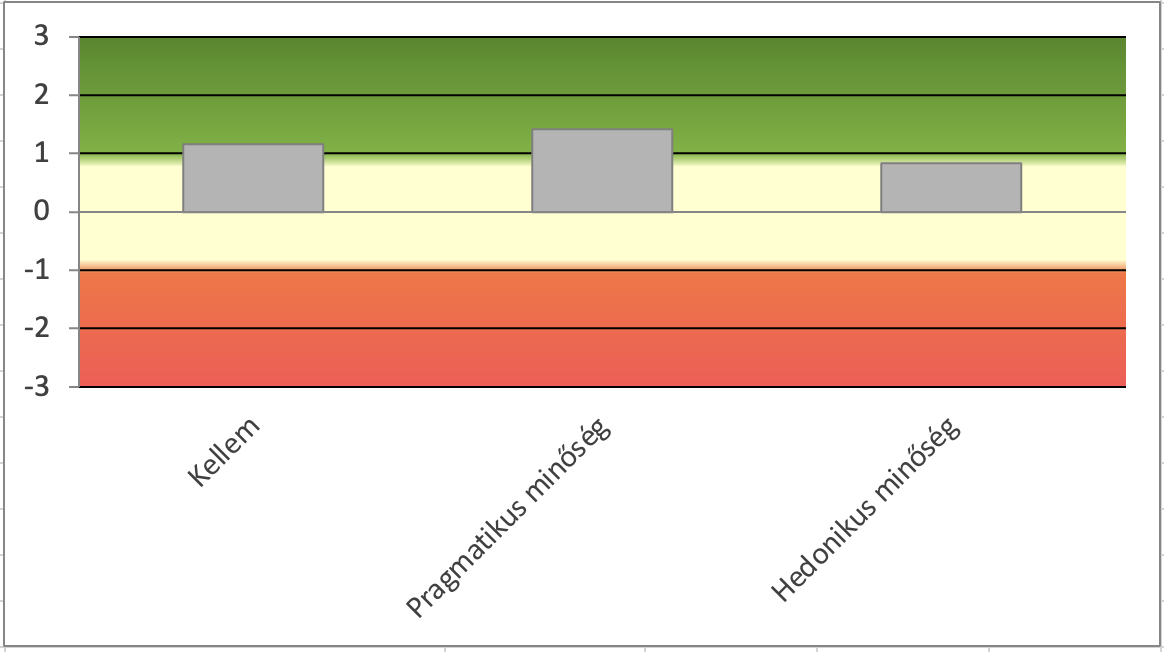
\includegraphics[width=0.75\textwidth]{img/UEQ_pragmatic_hedonic.png}
    \caption{Diagram: UEQ pragmatikus és hedonikus minőségek}
    \label{diag:pragmatic_hedonic}
\end{figure}

\section{SUS - System Usability Scale}

A SUS (System Usability Scale) egy rövid, 10 kérdésből álló kérdőív, amely a rendszerek, termékek vagy szolgáltatások használhatóságának gyors és hatékony értékelésére szolgál. A kérdőív célja, hogy visszajelzést adjon a felhasználói élményről és az általános elégedettségről.

\subsection{Működési Elv}
\begin{enumerate}
    \item \textbf{Kérdések:} A SUS kérdőív 10 állítást tartalmaz, amelyek a rendszer használhatóságával kapcsolatosak. A kérdések között találhatóak pozitív (pl. ``Azt hiszem, szeretném gyakran használni ezt a rendszert.'') és negatív (pl. ``Azt tapasztaltam, hogy a rendszer szükségtelenül bonyolult.'') megfogalmazású kijelentések.
    
    \item \textbf{Értékelés:} A válaszadók 5 pontos skálán (1-től 5-ig) értékelik az állításokat. A skála 1 = ``Teljesen nem értek egyet'' és 5 = ``Teljesen egyetértek'' közötti értékeket használja.
    
    \item \textbf{Számítás:} A válaszok értékelése során a pozitív állításoknál 1-gyel csökkentik a választ, majd ezt az értéket kivonják 5-ből. A negatív állításoknál a választ egyszerűen levonják 1-ből. A végső pontszám kiszámításához az összes állítás eredményeit összeadják, majd ezt az értéket megszorozzák 2.5-tel, így egy 0-tól 100-ig terjedő skálán kaphatunk eredményt.
    
    \item \textbf{Értelmezés:} Az így kapott pontszám segít a termék vagy rendszer használhatóságának általános értékelésében. A 68-as átlagpontszám körüli értékek a használhatóság jónak számítanak, míg az ennél alacsonyabb értékek problémákat jelezhetnek.
\end{enumerate}

\subsection{Kérdéseim és a válaszok}
A tíz kérdészem/kijelentésem, melyre pontot kellett adniuk, a következők voltak:

\begin{enumerate}
    \item Azt hiszem, szeretném gyakran használni ezt a rendszert.
    \item Azt tapasztaltam, hogy a rendszer szükségtelenül bonyolult.
    \item Úgy gondoltam, hogy a rendszer könnyen használható.
    \item Azt hiszem, szükségem lenne egy műszaki szakember támogatására ahhoz, hogy használni tudjam ezt a rendszert.
    \item Úgy találtam, hogy a rendszer különböző funkciói jól integráltak.
    \item Úgy éreztem, hogy túl sok ellentmondás van ebben a rendszerben.
    \item Azt képzelem, hogy a legtöbb ember nagyon gyorsan megtanulná használni ezt a rendszert.
    \item Azt tapasztaltam, hogy a rendszer nagyon nehézkes a használat során.
    \item Nagyon magabiztosan éreztem magam a rendszer használata közben.
    \item Sokat kellett tanulnom, mielőtt elkezdhettem volna használni ezt a rendszert.
\end{enumerate}

\begin{table}[h]
    \centering
    \begin{tabular}{|c|c|c|c|c|c|c|c|c|c|c|}
        \hline
        ID & 1 & 2 & 3 & 4 & 5 & 6 & 7 & 8 & 9 & 10 \\ \hline
        1  & 2 & 4 & 2 & 2 & 3 & 2 & 4 & 2 & 4 & 2  \\ \hline
        2  & 4 & 1 & 5 & 1 & 4 & 1 & 5 & 1 & 5 & 1  \\ \hline
        3  & 3 & 1 & 5 & 1 & 3 & 1 & 5 & 1 & 5 & 1  \\ \hline
        4  & 3 & 1 & 5 & 1 & 4 & 1 & 5 & 1 & 4 & 1  \\ \hline
        5  & 5 & 1 & 1 & 2 & 2 & 3 & 2 & 2 & 3 & 2  \\ \hline
        6  & 2 & 2 & 4 & 2 & 3 & 2 & 5 & 1 & 4 & 1  \\ \hline
        7  & 5 & 1 & 5 & 1 & 5 & 1 & 5 & 1 & 5 & 1  \\ \hline
        8  & 4 & 1 & 5 & 3 & 3 & 1 & 5 & 1 & 5 & 1  \\ \hline
        9  & 1 & 1 & 5 & 1 & 5 & 1 & 5 & 1 & 5 & 1  \\ \hline
        10 & 1 & 1 & 5 & 2 & 5 & 1 & 5 & 1 & 5 & 1  \\ \hline
        11 & 2 & 1 & 5 & 3 & 3 & 2 & 4 & 1 & 5 & 1  \\ \hline
    \end{tabular}
    \caption{Válaszok}
    \label{tab:sus_data}
\end{table}

A \url{https://sus.mixality.de/} eszközt használva a következő analízisek jöttek ki a \ref{tab:sus_data}. táblázat eredményeire. 

Az eredmények a következők: 
\begin{itemize}
    \item \textbf{SUS Tanulmány Pontszám:} 82.5
    \item \textbf{Medián:} 87.5
    \item \textbf{Szórás:} 14.19
    \item \textbf{Jellemző:} Kiváló
    \item \textbf{Osztályzat:} A
    \item \textbf{Elfogadhatóság:} Elfogadható
    \item \textbf{Negyed:} 4. negyed
\end{itemize}

\begin{figure}[h]
    \center
    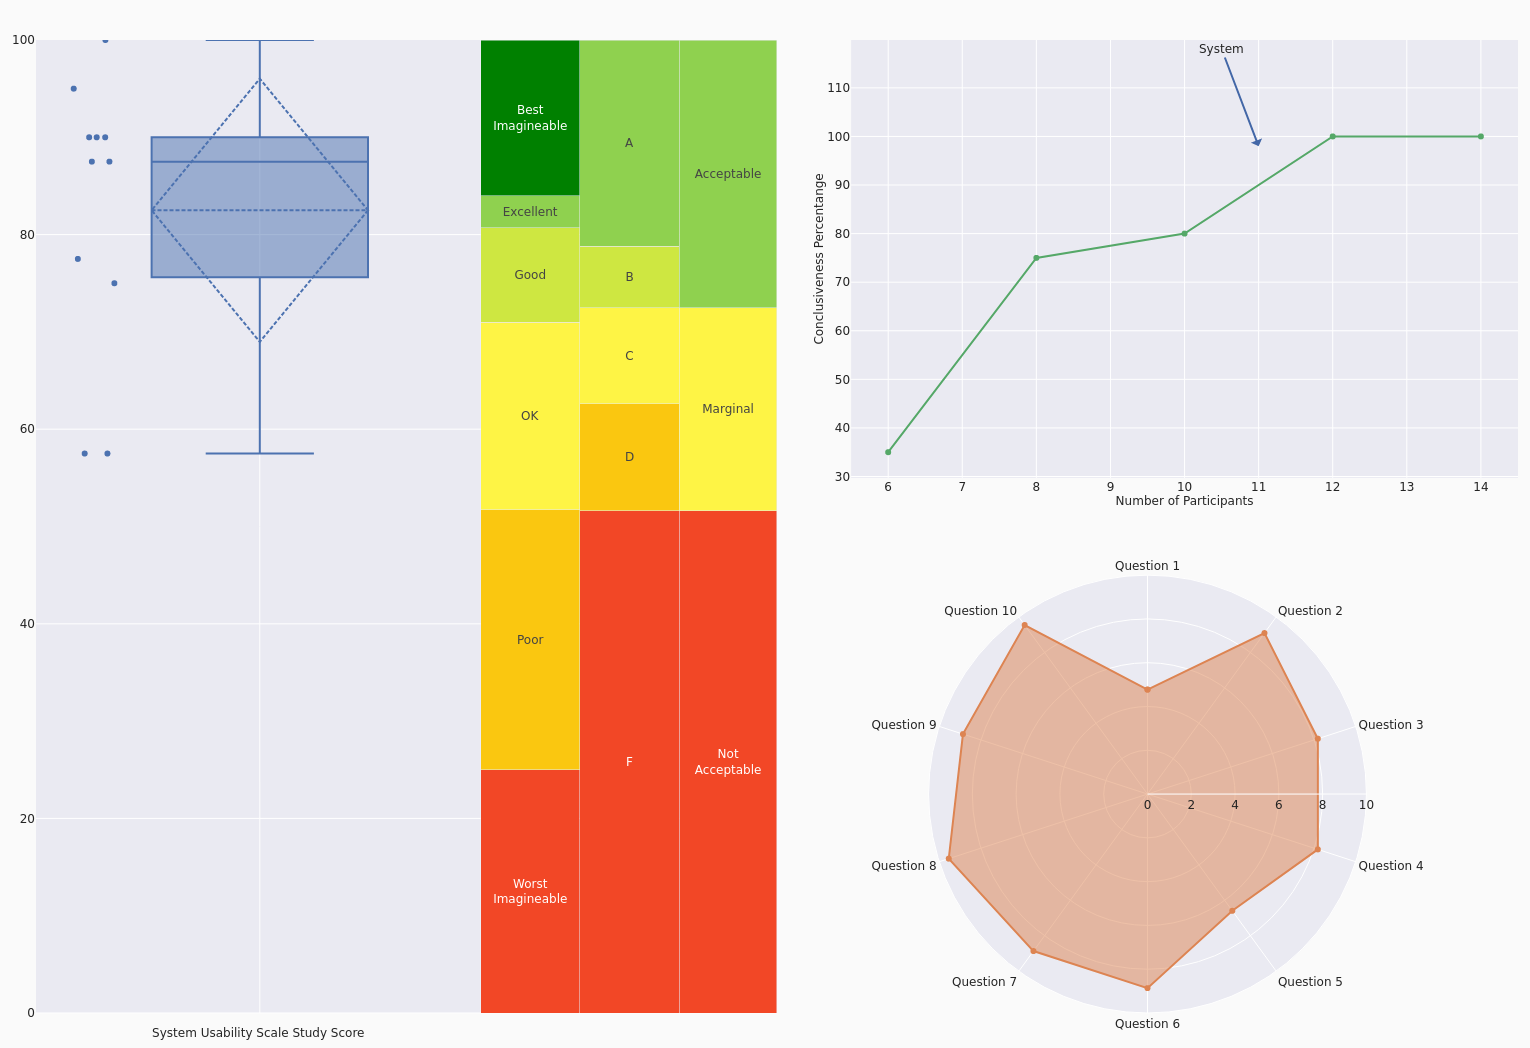
\includegraphics[width=\textwidth]{img/single_study_plot.png}
    \caption{SUS táblázat kiértékelt eredményei}
    \label{diag:sus_result}
\end{figure}

A diagrammon (\ref{diag:sus_result}. ábra) egyértelműen látszik, hogy az első és az ötödik kérdésekben a memória játékom alul teljesített. Az első kérdés, amely arra vonatkozik, hogy a felhasználók mennyire szeretnék gyakran használni a játékot, azt mutatja, hogy a válaszadók viszonylag alacsony érdeklődést mutatnak a rendszer rendszeres használata iránt. Ez aggasztó, mivel a gyakori használat egy fontos indikátora lehet a játék élvezhetőségének és vonzerejének.

Az ötödik kérdés kapcsán a felhasználók átlagos minőségűnek ítélték a megvalósítást, ami arra utal, hogy a játék nem hagyott maradandó benyomást, és nem tudta felkelteni a felhasználók érdeklődését olyan mértékben, hogy kiemelkedő minőséget mutasson. Ez a fajta közepes értékelés azt jelzi, hogy bár a játék elér egy bizonyos szintet, van még lehetőség a fejlődésre.

Mindkét területen – a felhasználói élmény fokozásában és a játék minőségének javításában – jelentős potenciál rejlik. Fontos lenne részletesen elemezni, hogy mik azok a konkrét elemek, amelyek nem nyerték el a felhasználók tetszését. Lehetséges, hogy a játékmenet, a grafika vagy akár a hangzásvilág is hozzájárulhat ehhez az érzéshez. A felhasználói visszajelzések figyelembevételével, valamint alapos tesztelésekkel képesek lehetünk a szükséges módosításokat végrehajtani, így a játék vonzereje és használhatósága jelentősen javulhat.

Ezeket a problémákat kezelve, a jövőbeni fejlesztések során érdemes lenne a felhasználói élményt középpontba állítani, hiszen egy élvezetes és vonzó játék ösztönözheti a felhasználókat a rendszeres visszatérésre és a játék gyakori használatára
